\documentclass[a4paper,11pt]{article}

%%%%%%%%%%%%%%%%%%%%%%%%%%%%%%%%%%%%%%%%%%%%%%%%%%%%%%%%%%%%%%%%%%%%%%%%
% Paquetes utilizados
%%%%%%%%%%%%%%%%%%%%%%%%%%%%%%%%%%%%%%%%%%%%%%%%%%%%%%%%%%%%%%%%%%%%%%%%

% Gráficos complejos
\usepackage{graphicx}
\usepackage{caption}
\usepackage{subcaption}
\usepackage{placeins}

% Soporte para el lenguaje español
\usepackage{textcomp}
\usepackage[utf8]{inputenc}
\usepackage[T1]{fontenc}
\DeclareUnicodeCharacter{B0}{\textdegree}
\usepackage[spanish]{babel}

% Código fuente embebido
\usepackage{listings}
\usepackage{courier}

% PDFs embebidos para el apéndice
\usepackage{pdfpages}

% Matemáticos
\usepackage{amssymb,amsmath}

% Tablas complejas
\usepackage{multirow}

% Formato de párrafo
\setlength{\parskip}{1ex plus 0.5ex minus 0.2ex}

% Formato de listados de código
\lstset{
  basicstyle=\footnotesize\ttfamily,
  numbers=left,
  numberstyle=\tiny,
  numbersep=5pt,
  tabsize=2,
  extendedchars=true,
  breaklines=true,
  frame=t,
  showspaces=false,
  showtabs=false,
  showstringspaces=false,
  language=Java,
  caption=\lstname,
  captionpos=t
}

%%%%%%%%%%%%%%%%%%%%%%%%%%%%%%%%%%%%%%%%%%%%%%%%%%%%%%%%%%%%%%%%%%%%%%%%
% Título
%%%%%%%%%%%%%%%%%%%%%%%%%%%%%%%%%%%%%%%%%%%%%%%%%%%%%%%%%%%%%%%%%%%%%%%%

% Título principal del documento.
\title{\textbf{Trabajo Práctico N°2}}

% Información sobre los autores.
\author{
  Andrés Gastón Arana(and2arana@gmail.com), \textit{P. 86.203}     \\
  Gabriel Ostrowsky(gaby.ostro@gmail.com), \textit{P. 90762}       \\
  Ignacio Garay Ojeda(imgarayojeda@gmail.com), \textit{P. 92265}   \\
  Pablo Angelani(pablo.angelani@gmail.com), \textit{P. 92707}      \\
  \normalsize{1er. Cuatrimestre de 2013}                           \\
  \normalsize{75.10 - Técnicas de Diseño}                          \\
  \normalsize{Facultad de Ingeniería, Universidad de Buenos Aires}
}
\date{}

%%%%%%%%%%%%%%%%%%%%%%%%%%%%%%%%%%%%%%%%%%%%%%%%%%%%%%%%%%%%%%%%%%%%%%%%
% Documento
%%%%%%%%%%%%%%%%%%%%%%%%%%%%%%%%%%%%%%%%%%%%%%%%%%%%%%%%%%%%%%%%%%%%%%%%

\begin{document}

% ----------------------------------------------------------------------
% Top matter
% ----------------------------------------------------------------------
\thispagestyle{empty}
\maketitle

\begin{abstract}

  Este informe sumariza el desarrollo del trabajo práctico grupal N°2 de la
  materia Técnicas de Diseño (75.10) dictada en el primer cuatrimestre de 2013
  en la Facultad de Ingeniería de la Universidad de Buenos Aires. El mismo
  consiste en el desarrollo de una aplicación minimalista para soportar las
  operaciones de una caja de una cadena de supermercados, aplicando los
  descuentos correspondientes vigentes al momento de la compra.

\end{abstract}

\clearpage

% ----------------------------------------------------------------------
% Tabla de contenidos
% ----------------------------------------------------------------------
\tableofcontents
\clearpage


% ----------------------------------------------------------------------
% Desarrollo
% ----------------------------------------------------------------------
\part{Desarrollo}

En esta sección se detallan algunas de las decisiones de diseño tomadas. Las
mismas tienen en cuenta la forma de proveer los Productos y Ofertas
disponibles, asi como también la implementación de las Ofertas Globales y
Exclusivas.  Para su implementación se tuvieron en cuenta las buenas prácticas
de programación, usando TDD en la medida de lo posible, criterios de buen
diseño y evitando bad-smells.  Además, se utilizaron algunos patrones vistos en
clase, detallados abajo.

A continuación se detallan los diferentes diagramas de clases correspondientes
a los distintos paquetes de la aplicación, como fue modelada, detallando
únicamente el modelo de dominio implementado.

\section{Caja}

El paquete de caja contiene todas las clases relacionadas con el manejo de la
caja propiamente dicha. En particular, algunas de las responsabilidades de las
clases de este paquete son el manejo de los estados de caja y la construcción
de nuevas instancias representativas de la compra a realizar por un cliente.

\begin{figure}[!htp]
\begin{center}
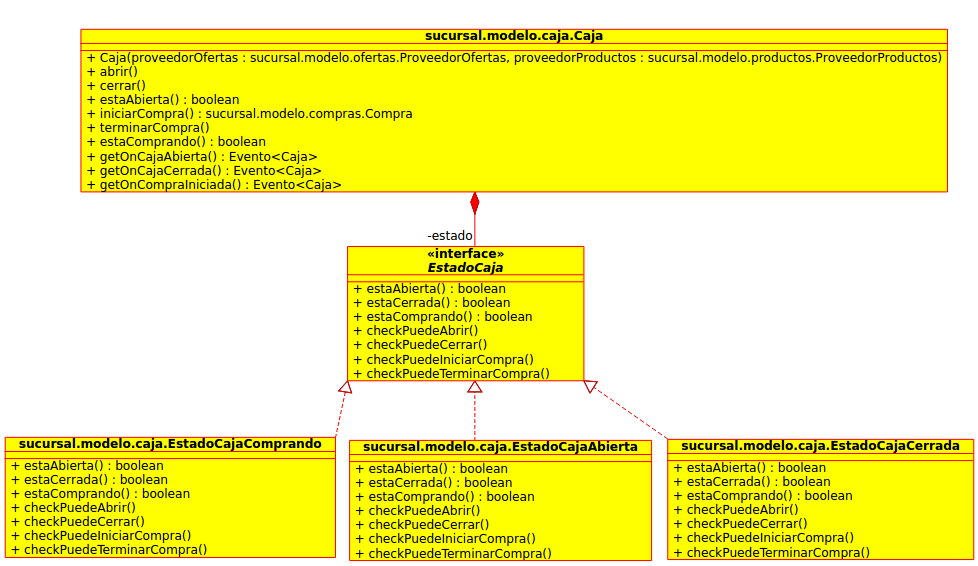
\includegraphics[width=1\textwidth]{src/docs/caja.png}
\end{center}
\caption{Diagrama de Clases} \label{fig:caja}
\end{figure}

\FloatBarrier

En la figura \ref{fig:caja} se detallan el diseño del paquete correspondiente.
Se puede observar la clase principal del paquete, Caja, que contiene la lógica
de intercambio de estados (abierta, cerrada y comprando). Este concepto de
estado se modeló utilizando el patrón State, como se puede apreciar en las
clases de EstadoCaja correspondientes. Cada estado es responsable de definir
los chequeos propios a las diferentes operaciones de la caja que corresponden a
los intercambios de estado de la misma.

Caja también recibe en su constructor dos objetos, ProveedorOfertas y
ProveedorProductos, encargados de proveerle las ofertas y productos del día al
momento de iniciar una nueva compra.

\section{Compra}

El paquete de compra contiene las clases relacionadas con la compra que realiza
el cliente, sirviendo como nodo de comunicación que utiliza las ofertas
(definidas en otro paquete) y los productos (en su propoi paquete también) para
representar la compra y los descuentos asociados a la misma.

\begin{figure}[!htp]
\begin{center}
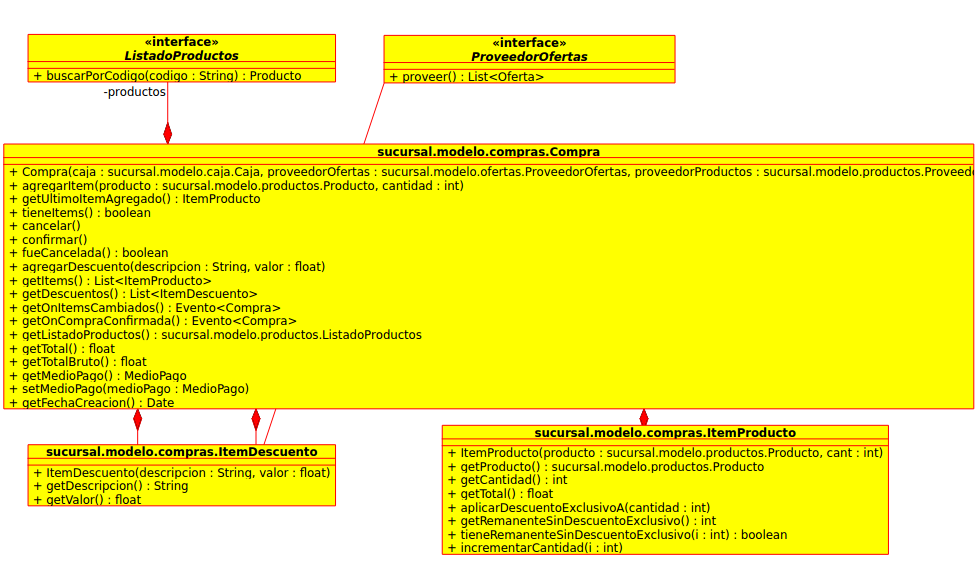
\includegraphics[width=1\textwidth]{src/docs/compras.png}
\end{center}
\caption{Diagrama de Clases} \label{fig:compra}
\end{figure}

\FloatBarrier

La clase principal del paquete, Compra, es la que representa el conjunto de
items comprados por un único cliente así como los descuentos aplicados. Consume
además los servicios del ListadoProducto y ProveedorOfertas para obtener los
productos en stock y las ofertas del momento en el que se inicia la compra.

Debido a que este paquete funciona como nodo central, integrando la
funcionalidad expuesta por otros paquetes (particularmente ofertas y
productos), intentamos mantener las interfaces entre ellos lo más acotadas
posible. La compra depende únicamente del Producto y de la Oferta propiamente
dicha, clases troncales de los paquetes correspondientes. El resto de los
servicios de dichos paquetes están ocultos, accedidos únicamente por las clases
del mismo paquete.

\section{Ofertas}

El paquete de ofertas contiene las clases relacionadas con el cálculo de los
descuentos apropiados a cada compra.

\begin{figure}[!htp]
\begin{center}
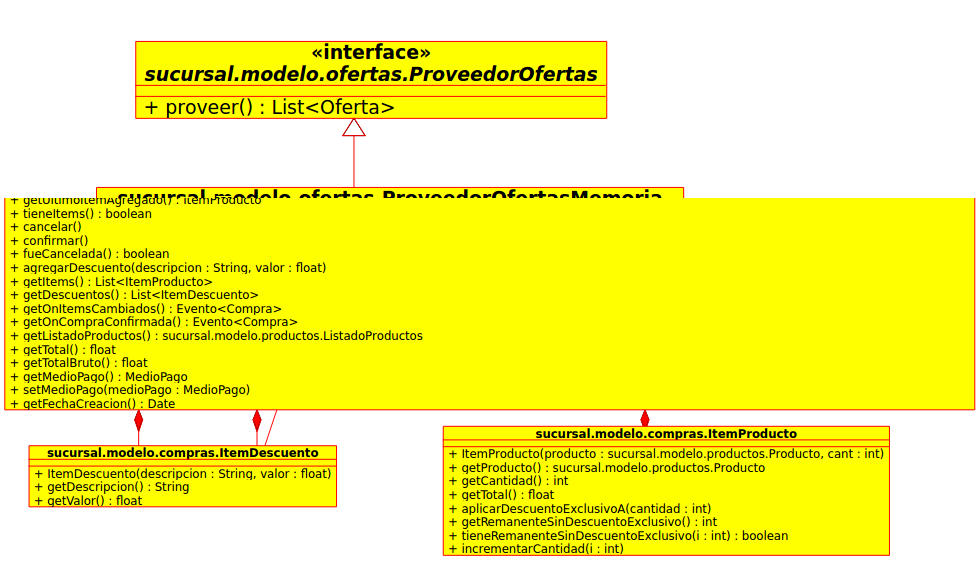
\includegraphics[width=1\textwidth]{src/docs/ofertas.png}
\end{center}
\caption{Diagrama de Clases} \label{fig:oferta}
\end{figure}

\FloatBarrier

La clase principal del paquete, Oferta, es la encargada de aplicar una oferta a
una compra. Para hacerlo, contiene referencias a dos interfaces, Predicate y
Function.

La interfaz Predicate es una interfaz genérica simple que, dado un objeto,
evalua una condicion y devuelve verdadero o falso. Oferta utiliza a Predicate
para evaluar si debe o no aplicar los descuentos asociados a la oferta.

La interfaz Function es una interfaz genérica, también simple, que transforma
una entidad en otro tipo de entidad. Esta interfaz se utiliza para dos
funciones: por un lado, permite implementar lógica de cálculo de los
descuentos, vista esta lógica como la conversión de una Oferta en un valor
decimal a descontar de la misma. Por el otro lado, esta interfaz permite
adaptar diferentes entidades de manera de poder reutilizar otras interfaces.

La eficacia de este diseño radica en la simplicidad de estas dos interfaces, lo
que posibilita su composición. Para dar un ejemplo, para definir una oferta que
aplique únicamente cuando el día actual es cierto día de la semana se definien
dos implementaciones de estas interfaces. La primera, una implementación de
Predicate que toma una fecha y evalua si la misma corresponde a un día de la
semana dado. La segunda, una implementación de Function que dado una compra
extrae y devuelve su fecha de creación. Componiendo estas dos interfaces se
obtiene un nuevo Predicate, que toma una Compra y evalúa si su fecha de
creación corresponde a un día de la semana dado.

En este aspecto, Predicate y Function funcionan como Composites, permitiendo la
definición flexible de los más diversos tipos de oferta con la mínima necesidad
de modificar el código existente.

\section{Consideraciones adicionales}

\subsection{Carga de Productos y Ofertas}

En relación al suministro de Productos disponibles a comprar y Ofertas vigentes
proveidas por la Sucursal, se utilizó una interfaz para las Cajas a modo de
obtener un listado de ambos objetos, sin importar el modo y formato de
persistencia de ambos catalogos.  En esta primera version del proyecto, se
crearon 2 clases de tipo Proveedores de Productos y Ofertas en Memoria, los
cuales implementan una interfaz para proveer el listado a la sucursal, y esta
asignarla a la caja.  A modo de demostración para su ejecución, armamos un
listado estatico de ambos elementos, con una variedad basica de productos entre
Marcas y Rubros, y ofertas Globales y Exclusivas.


\subsection{Condición de Ofertas Exclusivas}

Existe un supuesto a la asignación de ofertas exclusivas para los productos.
Estas ofertas, como es sabido, no pueden tener multiple asignación a un mismo
producto. Para implementarlo, incluímos un mecanismo que le permite a una
oferta marcar una cierta cantidad de items de la compra compo alcanzados por
una oferta exclusiva. Otras ofertas exclusivas pueden consultar esta marca para
detectar su aplicabilidad.

Implementamos únicamente una oferta exclusiva, del tipo "page X, lleve Y".
Consideramos que esta bastaba para demostrar el mecanismo de extensión que
permite definir más ofertas de este tipo sin impactar demasiado en el diseño.

Efectivamente, nuestro algoritmo de selección de las ofertas exclusivas para
los productos es asignar la primer oferta que cumple con todos los requisitos.

\clearpage

\part{Apéndice}
\appendix

\section{Enunciado original}\label{sec:enunciado}
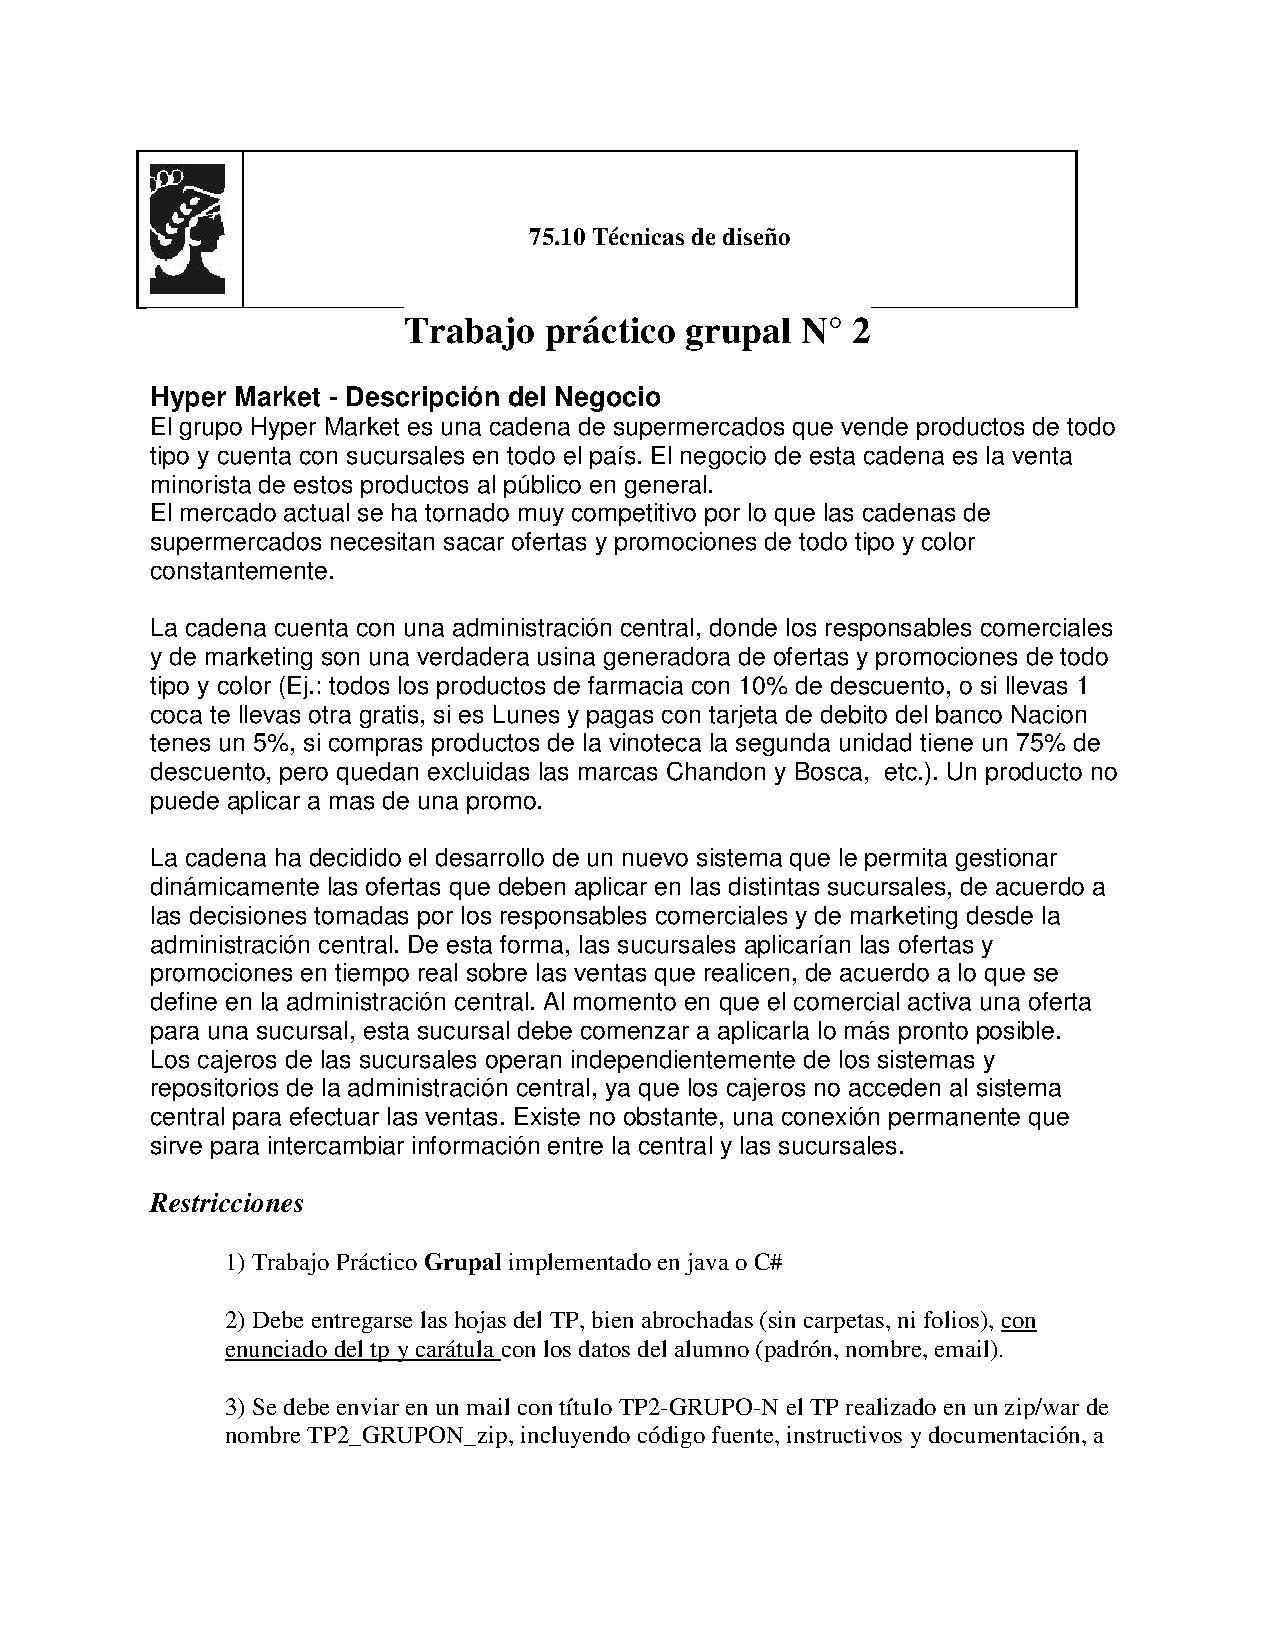
\includepdf[pages={-}, frame=true, pagecommand={}, noautoscale=true, scale=0.7]{src/docs/enunciado.pdf}

\end{document}

